

\begin{figure}
  \begin{center}
    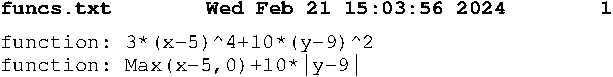
\includegraphics[width=0.95\textwidth]{funcs.pdf}
  \end{center}
  \caption{Two bivariate functions downloaded from \texttt{https://www.scss.tcd.ie/Doug.Leith/CS7DS2/week4.php}}\label{lst:funcs.txt}
\end{figure}


Let \begin{equation}
  f(x,y)=3(x-5)^4+10(y-9)^2
  \label{eq:f}
\end{equation}
and 
\begin{equation}
  g(x,y)=\max(x-5,0)+10|y-9|
  \label{eq:g}
\end{equation}

Using \texttt{sympy} we find the derivatives:
$$\nabla f=[\frac{df}{dx},\frac{df}{dy}]=[12(x-5)^{3},20y-180]$$
$$\nabla g=[\frac{dg}{dx},\frac{dg}{dy}]=[\text{Heaviside}(x-5),10\text{sign}(y-9)]$$


Clearly, the minimum of $f(x,y)$ is $0$ and they is minimized by $x=5$, $y=9$.
The other function $g(x,y)$ also has minimum $0$ but is minized by any of $x\in[-\infty,5]$ and $y=9$.


\begin{figure}
  \begin{center}
    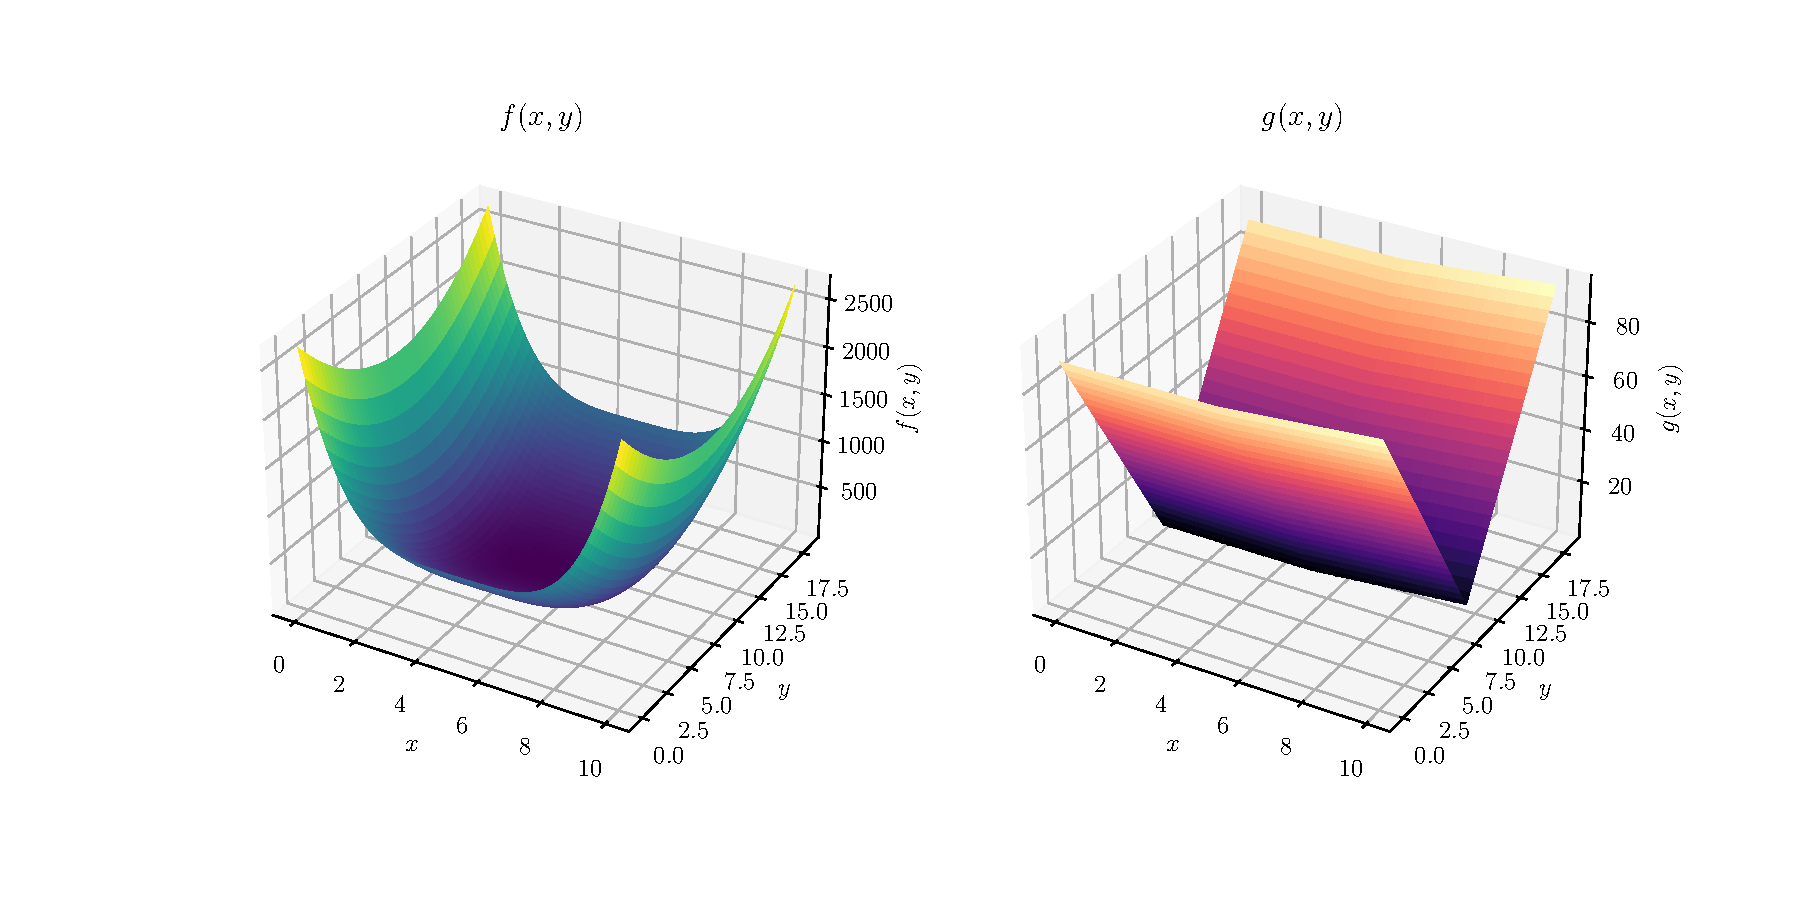
\includegraphics[width=0.95\textwidth]{fig/f-g.pdf}
  \end{center}
  \caption{}\label{fig:f-and-g}
\end{figure}

\section{(a)}
\subsection{(a) (i) Polyak}

The Polyak step size is
\begin{equation}
  \alpha_{\text{Polyak}}=\frac{f(x)-f^*}{\del f(x)^T\del f(x)}
  \label{eq:polyak-step}
\end{equation}
where $x$ is the parameter vector, $f(x)$ is the function to optimise, and $f^*\approx\min_xf(x)$.

Gradient descent iteration with Polyak step size is implemented in Listing~\ref{lst:polyak-implementation}.
The function is evaluated at the current value for $x$ and the numerator is calculated: $f(x)-f^*$.
A reasonable estimate for the minimum of the function, $f^*$, is required, here assumed to be $0$.
The dot product of the gradient is taken as the denominator. The step size is $\frac{f(x)-f^*}{\nabla f(x)^T\nabla f(x)}$.
We multiply the step size by the gradient and subtract the result from the current $x$.
\begin{listing}
  \begin{center}
    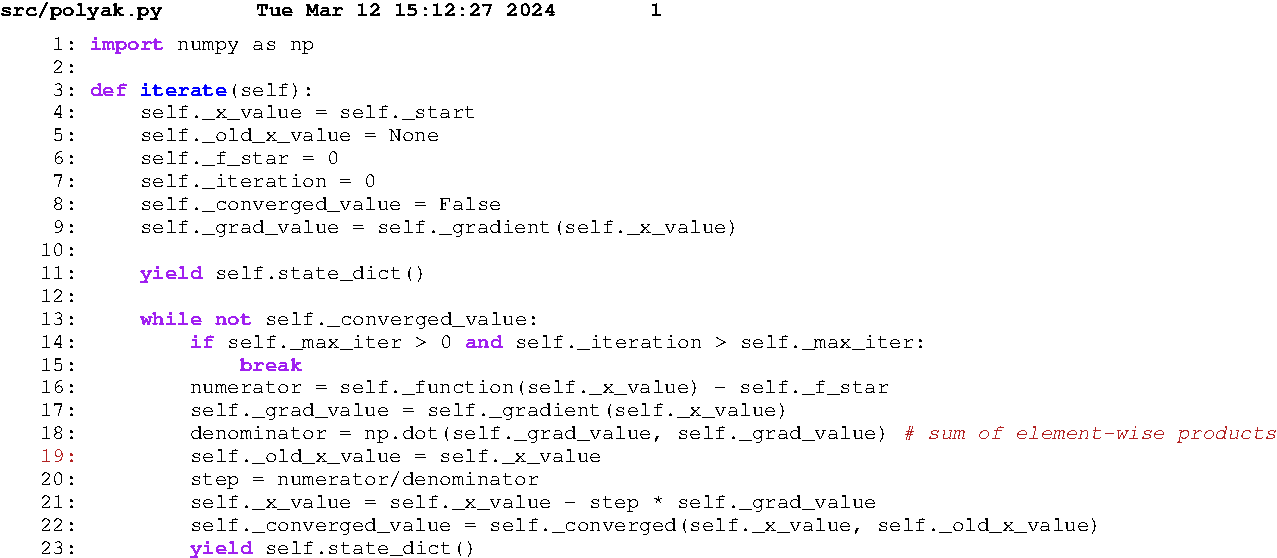
\includegraphics[width=0.95\textwidth]{fig/polyak-code.pdf}
  \end{center}
  \caption{An implementation of the update step of gradient descent using Polyak step size.}\label{lst:polyak-implementation}
\end{listing}

\subsection{(a) (ii) RMSProp}

The RMSProp step size at iteration $t$ is
\begin{equation}
  \alpha_t=\frac{\alpha_0}{\epsilon +
  \sqrt{(1-\beta)\sum_{i=0}^{t-1}\beta^{t-i}(\nabla f(x_i))^2}}
\end{equation}
and the update rule is \begin{equation}
  x_{t+1}:=x_t-\alpha_t*\nabla f(x_t)
\end{equation}
where $\epsilon$ is some small value to prevent divide by zero, $\alpha_0$
and $\beta$ are hyperparameters to be set, noting that $0<\beta\le1$. The
result is that previous gradients influence the current step size, but are
gradually forgotten due to the $\beta^{t-i}$ term.

A Python implementation of the update step is provided in
Listing~\ref{lst:rmsprop-implementation}. The term inside the square root
can be calculated iteratively, as in line 25 of
Listing~\ref{lst:rmsprop-implementation}.


\begin{listing}
  \begin{center}
    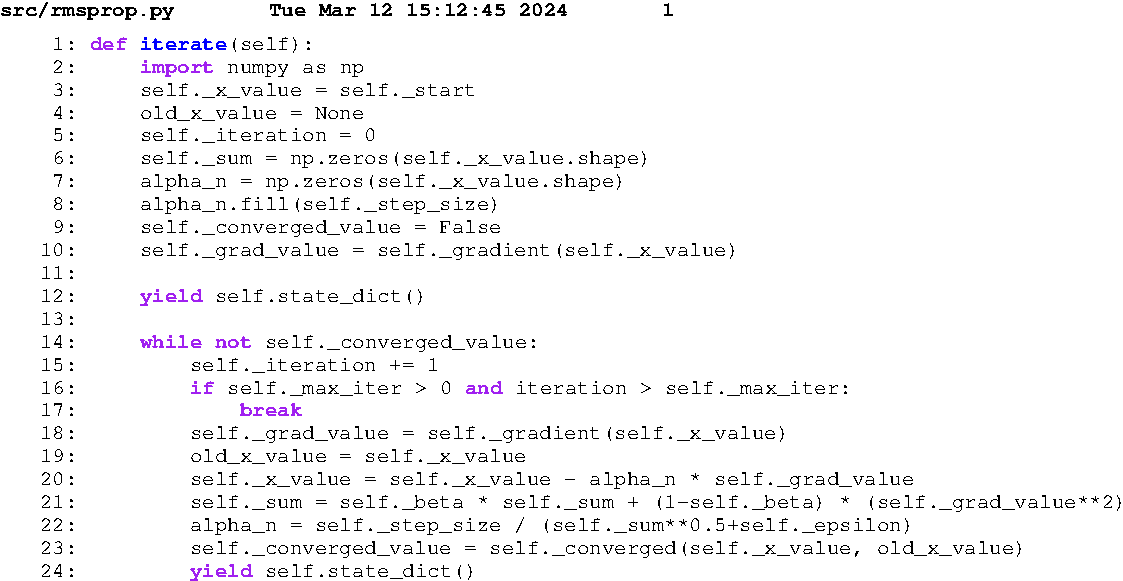
\includegraphics[width=0.95\textwidth]{fig/rmsprop-code.pdf}
  \end{center}
  \caption{An implementation of the update step of gradient descent using RMSProp step size.}\label{lst:rmsprop-implementation}
\end{listing}

\subsection{(a) (iii) Heavy Ball}

The Heavy Ball step is
\begin{equation}
  z_{t+1}=\beta z_t + \alpha\nabla f(x_t)
\end{equation}
with the update rule \begin{equation}
  x_{t+1}=x_t-z_{t+1}
\end{equation}
where t is the current iteration (starting at 0), $z_0=0$, and
$x_0$, $\alpha$, and $\beta$ have to be set.

A Python implementation of the update step is provided in Listing~\ref{lst:heavy_ball-implementation}.

\begin{listing}
  \begin{center}
    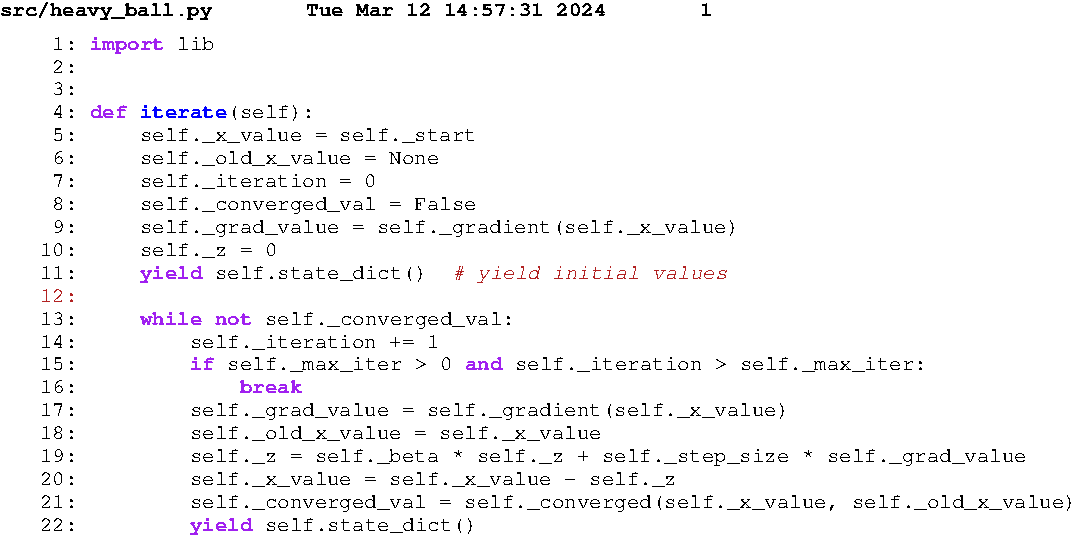
\includegraphics[width=0.95\textwidth]{fig/heavy_ball-code.pdf}
  \end{center}
  \caption{An implementation of the update step of gradient descent using Heavy Ball step size.}\label{lst:heavy_ball-implementation}
\end{listing}

\subsection{(a) (iv) Adam}

The Adam step size is calculated in terms of
\begin{equation}
  m_{t+1}=\beta_1m_t+(1-\beta_1)\nabla f(x_t)
\end{equation}
and \begin{equation}
  v_{t+1}=\beta_2v_t+(1-\beta_2)[\nabla f(x_t) \circ \nabla f(x_t)]
\end{equation}
from which we get
\begin{equation}
  \hat m=\frac{m_{t+1}}{(1-\beta_1^t)}
\end{equation}
and
\begin{equation}
  \hat v=\frac{m_{t+1}}{(1-\beta_2^t)}
\end{equation}
which are used in the update step as
\begin{equation}
  x_{t+1}=x_t-\alpha[\frac{\hat m_1}{\epsilon + \sqrt{\hat v_1}},\ldots,\frac{\hat m_n}{\epsilon + \sqrt{\hat v_n}}]
\end{equation}
where $t$ is the iteration, $\alpha$, $\beta_1$, and $\beta_2$ are hyperparameters, and $\epsilon$ is some small value to prevent divide-by-zero.

A Python implementation of the update step is provided in Listing~\ref{lst:adam-implementation}.

\begin{listing}
  \begin{center}
    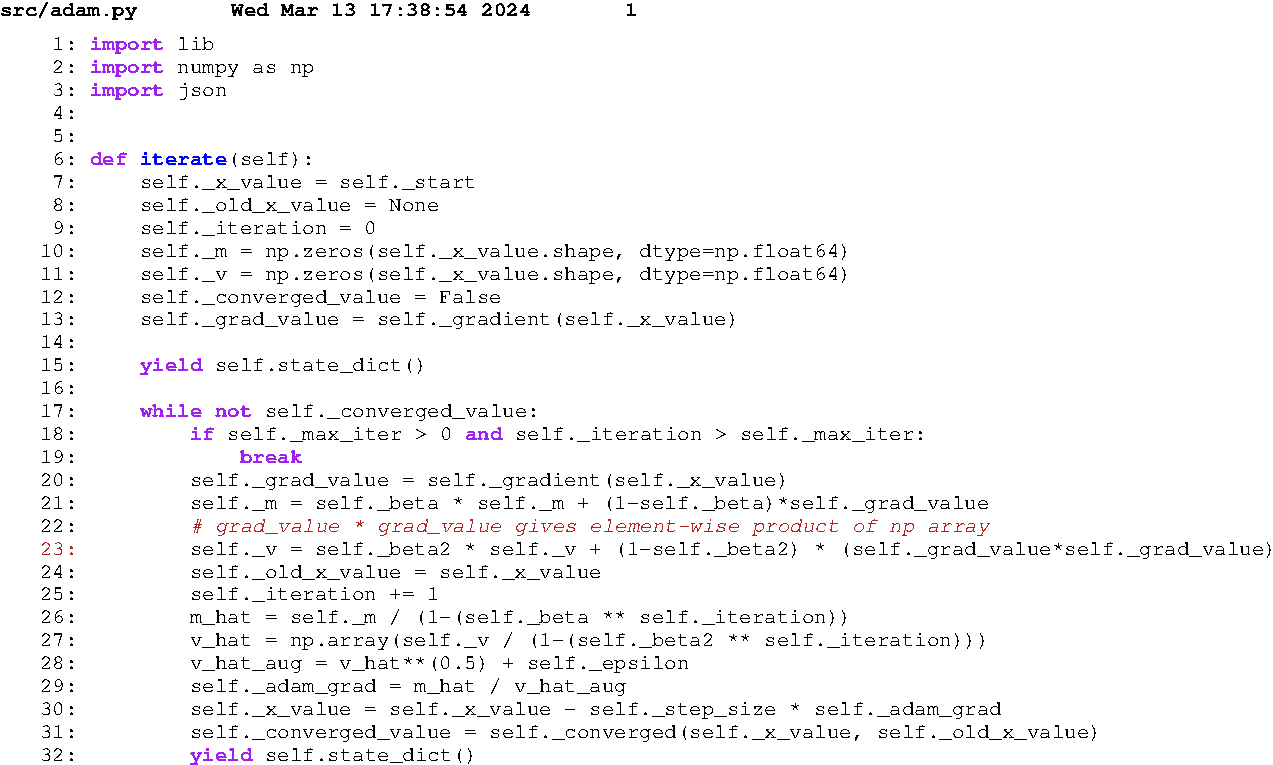
\includegraphics[width=0.95\textwidth]{fig/adam-code.pdf}
  \end{center}
  \caption{An implementation of the update step of gradient descent using Adam step size.}\label{lst:adam-implementation}
\end{listing}
